\documentclass[11pt]{article}
\usepackage[utf8]{inputenc}
\usepackage{amsmath}
\usepackage{amsfonts}
\usepackage{amssymb}
\usepackage{graphicx}
\usepackage[super]{nth}
\usepackage{amsthm}
\usepackage{bm}
\newtheorem{theorem}{Theorem}
\newtheorem{objective}{Objective}
\newtheorem{model}{Model}
\usepackage{xcolor}
\definecolor{light-gray}{gray}{0.95}
\newcommand{\code}[1]{\colorbox{light-gray}{\texttt{#1}}}
\usepackage{listings}
\usepackage{placeins}
\usepackage{enumitem}
\usepackage[T1]{fontenc}

\usepackage[authoryear]{natbib}

\lstset{language=R}


\makeatletter
\renewcommand{\maketitle}{
\begin{center}

\pagestyle{empty}

{\Large \bf \@title\par}
\vspace{1cm}

{\LARGE Marcel Gietzmann-Sanders}\\[1cm]

STAT651 - Statistical Theory I \\
University of Alaska Fairbanks


\end{center}
}\makeatother


\title{Homework 3}

\date{2025}
\setcounter{tocdepth}{2}
\begin{document}
\maketitle

\section{Question 1}

To have your game end after $n$ rolls you would need to have not gotten a 5 or a 6 $n-1$ times in a row. For each of these $n-1$ rolls the likelihood of not getting a 5 or a 6 is $4/6$. The likelihood of getting a 5 or 6 on a roll is $2/6$. Therefore, the likelihood of having to roll $n$ times before getting a 5 or a 6 is:

$$P(x=n)=(4/6)^{n-1}(2/6)$$

This also means that:

$$P(x\leq n) = \sum_{i=0}^{n-1}(4/6)^{i}(2/6)=(2/6)\sum_{i=0}^{n-1}(4/6)^{i}$$

Therefore:

$$P(x>3)=1-P(x\leq 3)=(2/6)=1-(2/6)\sum_{i=0}^{3-1}(4/6)^{i}\approx 0.2963$$

Therefore the probability that we need more that 3 tosses is 0.2963. 

$$P(x\leq 2)=(2/6)\sum_{i=0}^{2-1}(4/6)^{i}\approx 0.5556$$

Therefore the probability that we need at most 2 tosses is 0.5556. 

\section{Question 2}

We have $P(U|D)=0.87$, $P(U|!D)=0.73$, and $P(D)=0.53$ where $U$ is the belief that dog intelligence is underrated and $D$ corresponds to have one or more dogs. We want to know $P(D|U)$. By Bayes theorem we have:

$$P(D|U)=\frac{P(U|D)P(D)}{P(U)}$$

The only thing we are missing here is $P(U)$. Given $D$ and $!D$ form a partition:

$$P(U)=P(U|D)P(D) + P(U|!D)P(!D)=P(U|D)P(D) + P(U|!D)(1-P(D))$$
$$=0.87(0.53)+0.73(1-0.53)=0.8042$$

Therefore:

$$P(D|U)=\frac{0.87(0.53)}{0.8042}\approx 0.5734$$

That is, if you believe dog intelligence is underrated there is a 57.34\% probability that you own at least one dog.

\section{Question 3}

\subsection{a}

\textbf{Premise:} If $P(B)=1$ then $P(A|B)=P(A)$ for any event $A$. \newline

\textbf{Proof:} $P(A|B)=P(A \cap B)/P(B)$ which in this case is $ P(A|B)=P(A \cap B)$ given $P(B)=1$. Therefore what we'd like to prove is that $P(A \cap B) = P(A)$. 


Assume $P(A\cap B^C)> 0$ then that would mean that $P(B^C) > 0$ as $P(B^C)$ must be greater than or equal to the probability of $B^C$ intersected with some set. This in turn would mean that $P(S) = P(B)+P(B^C)>1$ which cannot be. Therefore $P(A\cap B^C)=0$. Given $P(A)=P(A \cap B) + P(A \cap B^C)$ we have $P(A)=P(A \cap B)$ and therefore that $P(A|B)=P(A \cap B)/P(B)=P(A|B)=P(A)/P(B)=P(A)$. 


\subsection{b}


\textbf{Premise:} If $A \subset B$ then $P(B|A) = 1$ and $P(A|B) = P(A)/P(B)$. \newline

\textbf{Proof:} If $A \subset B$ then $A \cap B = A$. Therefore $P(A \cap B) = P(A)$ which means that $P(A|B)=P(A \cap B)/P(B)=P(A)/P(B)$. Similarly $P(B|A)=P(A \cap B)/P(A) = P(A)/P(A)=1$. 

\subsection{c}

\textbf{Premise:} If $A$ and $B$ are mutually exclusive then:

$$P(A|A \cup B)= \frac{P(A)}{P(A) + P(B)}$$

\textbf{Proof:} A result we proved last homework is that:

$$P(A \cup B) = P(A) + P(B) - P(A \cap B)$$

However in this case $P(A \cap B)=P(\emptyset)=0$. Therefore $P(A \cup B) = P(A) + P(B)$. 

It is also true that $A \cap (A \cup B) = A$, therefore $P(A \cap (A \cup B)=P(A)$. 

So it follows that:

$$P(A|A \cup B)=\frac{P(A \cap (A \cup B)}{P(A \cup B)} = \frac{P(A)}{P(A) + P(B)}$$

\newpage

\section{Question 4}

\begin{figure}[h!] 
	\centering
  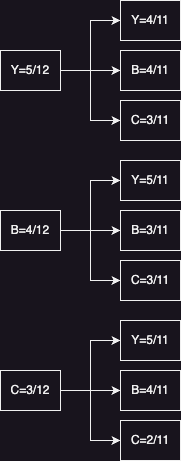
\includegraphics[height=75mm]{tree.png}
  \label{fig:tree}
\end{figure}

\FloatBarrier


\begin{enumerate}[label=\alph*]
\item P(Two Y's) $ = (5/12)(4/11)=20/132\approx 0.1515$
\item P(Different Colors) = 1 - P(Same Colors) $=1 - (5/12)(4/11) - (4/12)(3/11) - (3/12)(2/11)=94/132\approx 0.7121$
\item P( the second puppy is Y | the first puppy is C ) $=5/11 \approx 0.4545$
\item P(Same Colors) $=(5/12)(4/11) - (4/12)(3/11) - (3/12)(2/11)=38/132\approx 0.2879$
\item P( the first puppy is C | the second puppy is B ). First let's get P(second puppy is B) $=(5/12)(4/11) + (4/12)(3/11) + (3/12)(4/11) = 44/132$. Next let's get P( the first puppy is C and the second puppy is B ) $=(3/12)(4/11)=12/132$. Then P( the first puppy is C | the second puppy is B ) $=(12/132)/(44/132)=12/44 \approx 0.2727$
\item See above: $12/132\approx 0.0909$
\end{enumerate}

\newpage



\section{Question 5}

First of all there are 50 choose 6 (15890700) possible hands. This will be our denominator in each of these cases. 

\subsection{a}

\begin{enumerate}
\item Choose a denomination for your five of a kind - 10 options
\item Choose the singleton - 45 options (50 - the five of a kind)
\end{enumerate}

Total $=(10)45=450$. Our probability is therefore:

$$\frac{450}{15890700}\approx 2.831(10^{-5})$$

\subsection{b}

\begin{enumerate}
\item Choose a denomination for your four of a kind - 10 options
\item Choose the four - 5 choose 4 = 5 options
\item Choose a denomination for your pair - 9 options
\item Choose the pair - 5 choose 2 = 10 options
\end{enumerate}

Total $=(10)5(9)10=4500$. Our probability is therefore 

$$\frac{4500}{15890700}\approx 2.831(10^{-4})$$

\subsection{c}

\begin{enumerate}
\item Choose a denomination for your four of a kind - 10 options
\item Choose the four - 5 choose 4 = 5 options
\item Choose the denominations of our singletons - 9 choose 2 = 36 options
\item Choose the card for the first singleton - 5 options
\item Choose the card for the second singleton - 5 options
\end{enumerate}

Total $=(10)5(36)5(5)=78750$. Our probability is therefore 

$$\frac{78750}{15890700}\approx 4.956(10^{-3})$$

\subsection{d}

\begin{enumerate}
\item Choose a denomination for the pair - 10 options
\item Choose the pair - 5 choose 2 = 10 options
\item Choose the remaining denominations - 9 choose 4 = 126 options
\item For each singleton choose a card - $5^4=625$ options
\end{enumerate}

Total $=(10)10(126)625=7875000$. Our probability is therefore 

$$\frac{7875000}{15890700}\approx 0.4956$$

\subsection{e}

\begin{enumerate}
\item Choose your two denominations - 10 choose 2 = 45 options
\item Choose the cards for your first denomination - 5 choose 3 = 10 options
\item Choose the cards for your second denomination - 5 choose 3 = 10 options
\end{enumerate}

Total $=45(10)10=4500$. Our probability is therefore 

$$\frac{4500}{15890700}\approx 2.831(10^{-4})$$

\end{document}